I tansistore MOSFET (\emph{Metal-Oxide Semiconductor Field-Effect Transistor}) è un dispositivo elettronico utilizzato sia in circuiti digitali, principalmente come interruttore controllato in tensione, sia in circuiti analogici, come amplificatori di segnale o come ressitenze controllate in tensione.\\

\begin{figure}[H]
  \centering
  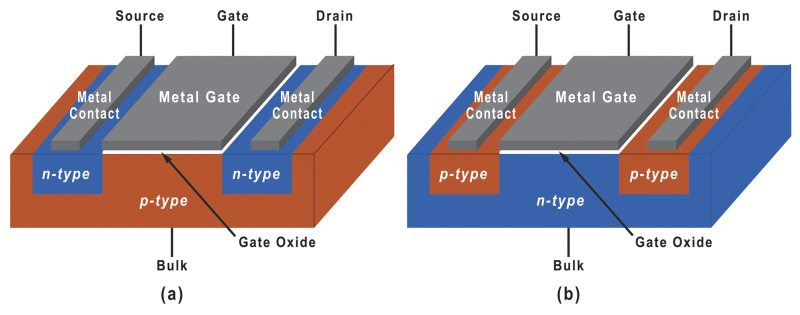
\includegraphics[width=0.80\textwidth]{./capitolo1/StrutturaMosfet}
  \caption[Struttura dei MOSFET]{MOSFET a canale N (a) e a canale P (b)}
  \label{fig:StrutturaMosfet}
\end{figure}

Come mostrato nella figura \ref{fig:StrutturaMosfet}, i MOSFET sono caratterizzati da quattro terminali: Source (S), Drain (D), Gate (G) e Bulk (B).
Il MOSFET a canale N viene realizzato su un substrato di tipo P in cui sono innestate due regioni fortemente drogate di tipo N. Queste due regioni presentano delle metallizzazioni che formano i terminali di Source e di Drain. Sul substrato, tra le due regioni fortemente drogate, è presente un sottile strato di ossido metallico che fa da isolante (storicamente $SiO_2$, attualmente si usano anche altri ossidi, più performanti) sopra il quale si trova una metallizzazione che forma il Gate. Il Bulk è il terminale che si collega direttamente con il substrato, sul lato opposto del Gate, e nella maggior parte dei casi è cortocircuitato con il Source, quindi non si considera.\\

\subsection{Regioni di funzionamento e caratteristica $I-V$}

\begin{figure}[H]
  \centering
  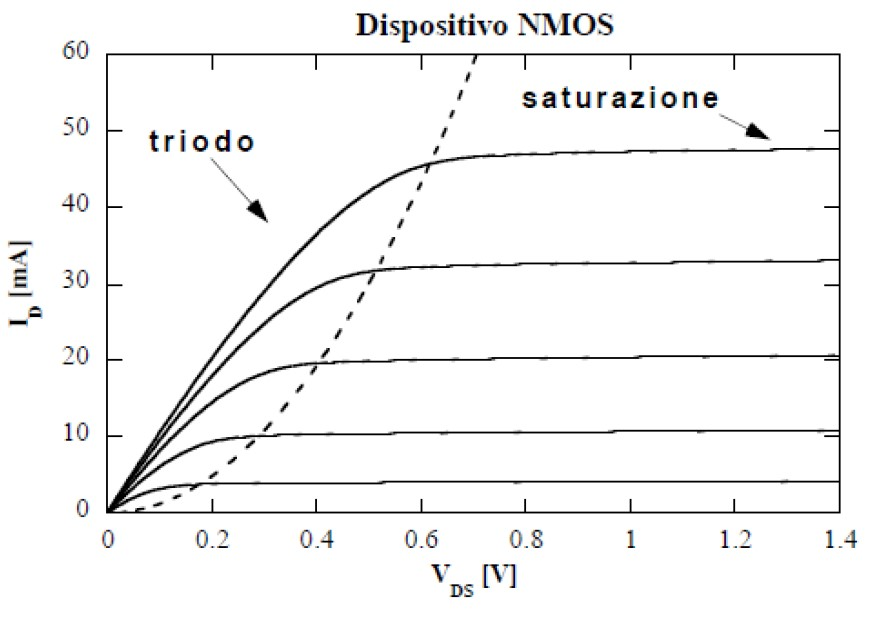
\includegraphics[width=0.80\textwidth]{./capitolo1/Caratteristica-I-V}
  \caption[Caratteristica $I-V$ di un MOSFET a canale N]{Caratteristica $I-V$ di un MOSFET a canale N}
  \label{fig:caratteristica-I-V}
\end{figure}

In un MOSFET a canale N, in linea generale, può scorrere una corrente $I_D$ che va dal Drain al Sourse in funzione di due tensioni (sempre non negative): 
\begin{itemize}
  \item la tensione presente tra Drain e Sourse ($V_{DS}$);
  \item la tensione presente tra Gate e Sourse ($V_{GS}$).  
\end{itemize}

La dipendenza di $I_D$ da tali tensioni è messa in evidenza dalla carattteristica corrente-tensione (figura \ref{fig:caratteristica-I-V}).

Quando $V_{GS} = 0$, indipendentemente dal valore di $V_{DS}$, la corrente $I_D$ è nulla, poiché le due giunzioni P-N, sono in regione inversa. \\
Aumentando il valore di $V_{GS}$, lacune si allontanano dalla regione direttamente al di sotto dell'ossido, creando una
zona svuotata di portatori di carica liberi. Gli elettroni presenti nel semiconduttore
vengono attirati creando una regione di canale di tipo N che unisce il
source e il drain. Questo canale permette il passaggio di corrente, ma per crearlo è necessario che $V_{GS}$ abbia un valore almeno pari alla cosiddetta tensione di soglia ($V_{th}$). Finché $V_{GS} < V_{th}$, il MOSFET si trova in regione di \emph{cutoff} e $I_D \simeq 0$.

Nel momento in cui $V_{GS}$ eguaglia e supera $V_{th}$, il canale di conduzione è completo e inizia a scorrere corrente, seguendo leggi matematiche differenti in funzione del valore di $V_{DS}$.\\

Se $V_{DS} < V_{GS} -  V_{th}$, il MOSFET è in regione lineare o di triodo e la corrente di Drain seue le seguente legge:\\
\centerline{ $I_D = 2k_n\left[ \left(V_{GS}-V_{th}\right)V_{DS} - \frac{V_{DS}^2}{2}\right]$}
con \\
dove
%%\begin{cases}
  %%$k_n$ & =  $\frac{1}{2}\mu_n C_{ox}\frac{W}{L}$ \\
  %%$\mu_n $ & = mobilità degli elettroni \\
  %%$C_{ox}$ &= capacità dell'ossido \\
  %%$W$ & = spessore del canale \\
  %%$L$ & = larghezza del canale \\
%%\end{cases}

Se, invece, $V_{DS} > V_{GS} -  V_{th}$ il MOSFET si trova in regione di saturazione e la corrente di drain ha un andamento lineare che segue la legge:\\
\centerline{ $I_D = k_n\left(V_{GS}-V_{th}\right)^2 (1+\lambda V_{DS}$}\\
dove $\lambda$ è un fattore matematico ricavato dalla caratteristica I-V ottenuta sperimentalmente.







